% =============================================================================
%  SAMPLE COMPANION  —  SMOKE TEST & QUALITY BAR  (standalone, compilable)
% =============================================================================
%  This is a SHORT (~2 page) fully-filled specimen companion for ONE topic:
%      "Poisson: counting rare events".
%  It re-declares a MINIMAL preamble that defines the FIVE callout boxes inline,
%  so a student can compile THIS file directly as a smoke test of the toolchain
%  and the house design — no external PNG, no project preamble required.
%
%  BUILD:
%      latexmk -pdf sample_companion.tex
%      # or twice (header/hyperref):
%      pdflatex sample_companion.tex && pdflatex sample_companion.tex
%
%  WHAT IT DEMONSTRATES (the bar every real companion must clear):
%      * the navy full-width title banner (page 1)
%      * the "How to use this companion." colour-code intro
%      * a NUMBERED, ruled section heading
%      * ALL FIVE callout boxes, each with its pill tab + glyph + tint
%      * a FULLY worked example — every algebraic step, real numbers
%      * one self-contained TikZ mini-figure (no external image)
%      * easy language, short sentences, every symbol named
% =============================================================================
\documentclass[a4paper,11pt]{article}

% ---- Encoding & fonts -------------------------------------------------------
\usepackage[T1]{fontenc}
\usepackage[utf8]{inputenc}
\usepackage{lmodern}
\usepackage{microtype}            % subtle protrusion -> fewer overfull boxes

% ---- Geometry ---------------------------------------------------------------
\usepackage[a4paper,margin=1in,headheight=15pt]{geometry}

% ---- Math, tables, graphics -------------------------------------------------
\usepackage{amsmath,amssymb,mathtools}
\usepackage{booktabs}
\usepackage{graphicx}
\usepackage{adjustbox}
\usepackage[dvipsnames,svgnames,table]{xcolor}

% ---- Dingbat glyphs for the pill tabs (portable, no Unicode font needed) ----
\usepackage{pifont}               % \ding{...} -> hand, star, pencil, cross, check

% ---- Callout boxes (breakable!) ---------------------------------------------
\usepackage[most]{tcolorbox}
\tcbuselibrary{skins,breakable}

% ---- Lists, spacing ---------------------------------------------------------
\usepackage{enumitem}
\setlist{leftmargin=1.5em,topsep=4pt,itemsep=3pt}
\usepackage{parskip}

% ---- TikZ for the mini-figure ----------------------------------------------
\usepackage{tikz}
\usetikzlibrary{arrows.meta}

% ---- Headers / footers ------------------------------------------------------
\usepackage{fancyhdr}

% ---- Links ------------------------------------------------------------------
\usepackage[hidelinks]{hyperref}
\usepackage{xurl}
\hypersetup{breaklinks=true}

% =============================================================================
%  TAXONOMY COLOURS  (the gold-standard companion palette)
% =============================================================================
\definecolor{navy}{HTML}{21355E}        % title-banner navy
\definecolor{cIntu}{HTML}{2C5AA0}       % blue  — The intuition
\definecolor{cEvery}{HTML}{8A5A1E}      % amber — Everyday picture
\definecolor{cWork}{HTML}{2E7D52}       % green — Worked example
\definecolor{cWatch}{HTML}{B23A48}      % red   — Watch out
\definecolor{cKey}{HTML}{6A4C93}        % purple— Key takeaway

% Very light tint fills (the "fill blue!4 / orange!7 / ..." equivalents).
\definecolor{cIntuBg}{HTML}{F4F7FC}
\definecolor{cEveryBg}{HTML}{FBF1E3}
\definecolor{cWorkBg}{HTML}{F1F8F3}
\definecolor{cWatchBg}{HTML}{FBF1F2}
\definecolor{cKeyBg}{HTML}{F5F1FA}

\definecolor{cInk}{HTML}{1A1A1A}        % body ink

% =============================================================================
%  CALLOUT BUILDER + THE FIVE BOXES
%  Pill tab sits on the top-left edge: boxed title attached
%  {xshift=6mm,yshift=-3mm}, solid colour, rounded, white bold sans text.
% =============================================================================
\newtcolorbox{calloutbox}[3]{%
  % #1 = accent colour (frame + pill), #2 = light tint fill, #3 = pill label
  enhanced, breakable,
  colback=#2, colframe=#1,
  boxrule=0.6pt, arc=2.5pt, outer arc=2.5pt,
  left=10pt, right=10pt, top=10pt, bottom=9pt,
  before skip=11pt, after skip=11pt,
  fonttitle=\bfseries\sffamily\small, coltitle=white,
  attach boxed title to top left={xshift=6mm,yshift=-3mm},
  boxed title style={colback=#1, colframe=#1, rounded corners,
                     boxrule=0pt, left=5pt, right=5pt, top=2pt, bottom=2pt},
  title={#3}%
}

% \ding{43}=hand index, {72}=star, {46}=pencil, {55}=cross, {52}=check.
\newenvironment{intuitionbox}{%
  \begin{calloutbox}{cIntu}{cIntuBg}{\ding{43}\, The intuition}}{\end{calloutbox}}
\newenvironment{everydaybox}{%
  \begin{calloutbox}{cEvery}{cEveryBg}{\ding{72}\, Everyday picture}}{\end{calloutbox}}
% Worked example takes a caption argument shown in the pill: "Worked example: ...".
\newenvironment{workedbox}[1]{%
  \begin{calloutbox}{cWork}{cWorkBg}{\ding{46}\, Worked example: #1}}{\end{calloutbox}}
\newenvironment{watchoutbox}{%
  \begin{calloutbox}{cWatch}{cWatchBg}{\ding{55}\, Watch out}}{\end{calloutbox}}
\newenvironment{keytakebox}{%
  \begin{calloutbox}{cKey}{cKeyBg}{\ding{52}\, Key takeaway}}{\end{calloutbox}}

% ---- Worked-example step list (numbered, breakable) -------------------------
\newlist{steps}{enumerate}{1}
\setlist[steps]{label=\textbf{Step \arabic*.},leftmargin=2.4em,topsep=4pt,itemsep=5pt}

% =============================================================================
%  NUMBERED, RULED SECTION HEADINGS (sans, navy)
% =============================================================================
\usepackage{titlesec}
\titleformat{\section}
  {\sffamily\bfseries\large\color{navy}}{\thesection}{1em}{}[{\color{navy!35}\titlerule[0.8pt]}]
\titlespacing*{\section}{0pt}{14pt}{6pt}

% =============================================================================
%  HEADER / FOOTER  (fancyhdr): "ISM Companion" left, session+title right.
% =============================================================================
\pagestyle{fancy}
\fancyhf{}
\renewcommand{\headrulewidth}{0.4pt}
\lhead{\sffamily\footnotesize\color{navy}ISM Companion}
\rhead{\sffamily\footnotesize\color{navy}Session 7 \textperiodcentered\ The Poisson Distribution}
\cfoot{\sffamily\footnotesize\thepage}

\color{cInk}
\begin{document}

% ----------------------------- TITLE BANNER ---------------------------------
\begin{tcolorbox}[enhanced, colback=navy, colframe=navy, boxrule=0pt,
                  arc=3pt, left=16pt, right=16pt, top=14pt, bottom=14pt,
                  coltext=white, width=\linewidth]
  {\sffamily\footnotesize\color{white!82}%
    \MakeUppercase{Introduction to Statistical Methods \textperiodcentered\ Companion Reader}}\\[8pt]
  {\sffamily\bfseries\Huge Poisson: counting rare events}\\[5pt]
  {\sffamily\large\color{white!88}%
    The distribution of "how many happened" when each one is rare.}\\[9pt]
  {\color{white!55}\rule{\linewidth}{0.4pt}}\\[6pt]
  {\sffamily\footnotesize\color{white!88}%
    Session 7 (6th--7th June 2026) \textperiodcentered\ Read alongside the lecture
    slides \textperiodcentered\ Every slide example worked out in full}
\end{tcolorbox}

\medskip
\noindent\textbf{How to use this companion.}
The slides give you the formulas; this reader gives you the \emph{why}. Read it
next to the deck. Five coloured boxes guide you. The blue
\textbf{\textcolor{cIntu}{intuition}} box explains an idea in plain words. The
amber \textbf{\textcolor{cEvery}{everyday picture}} box ties it to real life. The
green \textbf{\textcolor{cWork}{worked example}} box solves a problem with real
numbers, every step shown. The red \textbf{\textcolor{cWatch}{watch out}} box flags
a common mistake. The purple \textbf{\textcolor{cKey}{key takeaway}} box is the
one line to remember.

% ============================================================================
\section{The big idea: counting rare events in a fixed window}
% ============================================================================

A \emph{Poisson distribution} answers one question: in a fixed stretch of time
or space, how many times does a rare event happen? Think of calls to a help
desk in one hour, or typos on one page. We do not ask \emph{when} each one
happens. We only count \emph{how many}.

The whole distribution rides on a single number, $\lambda$ (the Greek letter
"lambda"). Here $\lambda$ is the \textbf{average count} you expect in that
window. If a help desk gets $3$ calls per hour on average, then $\lambda = 3$
for a one-hour window. That is all you need.

\begin{intuitionbox}
Picture a long, quiet afternoon at a shop. Customers trickle in at random.
There is no schedule and no pattern. You cannot say "the next one comes at
2:40". But you \emph{can} say "about $4$ per hour, on average". The Poisson
distribution turns that one average, $\lambda$, into the full odds: the chance
of seeing exactly $0$, exactly $1$, exactly $2$ customers, and so on. One
number in; a whole table of probabilities out.
\end{intuitionbox}

\begin{everydaybox}
Think of rain hitting a single floor tile during a light drizzle. Drops land at
random spots and random moments. Stand over one tile for ten seconds and count
the hits. Some ten-second spells catch $0$ drops, some catch $1$, a few catch
$3$ or $4$. The \emph{average} hits per ten seconds is steady; the
\emph{exact} count jumps around. That jumpy count is exactly a Poisson count.
\end{everydaybox}

Now the formula. The probability of seeing exactly $k$ events is
%
\begin{equation}
  P(X = k) \;=\; \frac{\lambda^{k}\, e^{-\lambda}}{k!},
  \qquad k = 0, 1, 2, \dots
  \label{eq:poisson}
\end{equation}
%
Let us name every symbol, slowly:
\begin{itemize}
  \item $X$ is the random count — the number we do not yet know.
  \item $k$ is one specific count we ask about, like "exactly $2$".
  \item $\lambda$ is the average count in the window (here, a positive number).
  \item $e \approx 2.71828$ is Euler's number, a fixed constant.
  \item $k! = k \times (k{-}1) \times \cdots \times 2 \times 1$ is "$k$
        factorial", and we set $0! = 1$ by convention.
\end{itemize}

\noindent Two facts make this easy to use. For a Poisson count, the
\textbf{mean} (average) and the \textbf{variance} (spread) are \emph{both} equal
to $\lambda$:
%
\begin{equation}
  \mathbb{E}[X] = \lambda,
  \qquad
  \operatorname{Var}(X) = \lambda .
  \label{eq:meanvar}
\end{equation}
%
So one number sets both the centre and the width of the distribution.

% ----------------------------- WORKED EXAMPLE -------------------------------
\begin{workedbox}{help-desk calls in one hour}
A help desk receives $\lambda = 3$ calls per hour on average. What is the
probability of getting \emph{exactly} $2$ calls in the next hour? Then, what is
the probability of getting \emph{at least} $1$ call?
\begin{steps}
  \item \textbf{Write down what we know.} The average is $\lambda = 3$. We want
        $P(X = 2)$, so the specific count is $k = 2$.
  \item \textbf{Plug into the formula \eqref{eq:poisson}.} Substituting
        $\lambda = 3$ and $k = 2$:
        \[
          P(X = 2) = \frac{3^{2}\, e^{-3}}{2!}.
        \]
  \item \textbf{Work out each piece.} The top has $3^{2} = 9$. The factorial is
        $2! = 2 \times 1 = 2$. The constant is $e^{-3} \approx 0.049787$.
  \item \textbf{Combine the numbers.}
        \[
          P(X = 2)
          = \frac{9 \times 0.049787}{2}
          = \frac{0.448083}{2}
          = 0.224042.
        \]
        So there is about a $\mathbf{22.4\%}$ chance of exactly two calls.
  \item \textbf{Now the "at least one" part.} "At least $1$" is the opposite of
        "exactly $0$". So compute $P(X = 0)$ first and subtract from $1$:
        \[
          P(X = 0) = \frac{3^{0}\, e^{-3}}{0!}
                   = \frac{1 \times 0.049787}{1}
                   = 0.049787.
        \]
  \item \textbf{Subtract.}
        \[
          P(X \ge 1) = 1 - P(X = 0)
                     = 1 - 0.049787
                     = 0.950213.
        \]
        So there is about a $\mathbf{95.0\%}$ chance of \emph{at least} one call.
\end{steps}
Notice the "at least" trick: instead of adding up $P(1) + P(2) + P(3) + \cdots$
forever, we used one easy subtraction. That shortcut works whenever "at least
one" is the goal.
\end{workedbox}

\begin{watchoutbox}
$\lambda$ must match your \emph{window}. The $3$ calls were \emph{per hour}. If
you ask about a $20$-minute window instead, scale $\lambda$ to that window
first: $20$ minutes is $\tfrac{1}{3}$ of an hour, so use $\lambda = 3 \times
\tfrac{1}{3} = 1$. Plugging the hourly $\lambda = 3$ into a $20$-minute question
silently inflates every probability. Always rescale $\lambda$ to the window you
are actually asking about.
\end{watchoutbox}

% ----------------------------- TIKZ MINI-FIGURE -----------------------------
\begin{center}
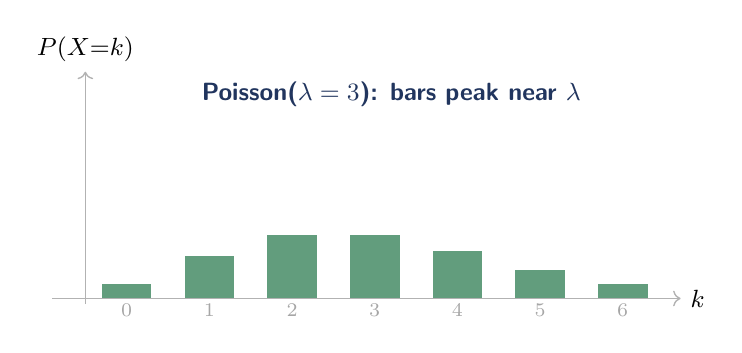
\begin{tikzpicture}[x=1.05cm,y=3.6cm]
  % axes
  \draw[->,gray!60,line width=0.5pt] (-0.4,0) -- (7.2,0) node[right,black,font=\small]{$k$};
  \draw[->,gray!60,line width=0.5pt] (0,-0.02) -- (0,0.80) node[above,black,font=\small]{$P(X{=}k)$};
  % Poisson(3) bars, heights = probabilities, drawn to scale (max ~0.224 at k=2,3)
  \foreach \k/\p in {0/0.0498,1/0.1494,2/0.2240,3/0.2240,4/0.1680,5/0.1008,6/0.0504}{
    \fill[cWork!75] (\k+0.20,0) rectangle (\k+0.80,\p);
    \node[font=\scriptsize,gray!70] at (\k+0.5,-0.04) {\k};
  }
  \node[font=\small\sffamily,navy] at (3.7,0.72) {\textbf{Poisson($\lambda=3$): bars peak near $\lambda$}};
\end{tikzpicture}
\end{center}

\noindent The bars are tallest around $k = 2$ and $k = 3$, right next to the
average $\lambda = 3$, then fade out for large $k$. A rare-event count clusters
near its mean and rarely strays far.

\begin{keytakebox}
One number, $\lambda$, is the whole story. It is the average count, and (by
\eqref{eq:meanvar}) also the variance. Feed it into
$P(X{=}k)=\lambda^{k}e^{-\lambda}/k!$ to get the chance of any exact count.
Always match $\lambda$ to your window, and use the "$1 - P(0)$" trick for "at
least one".
\end{keytakebox}

% ----------------------------- ML/AI CONNECTION -----------------------------
\noindent\textbf{Where this shows up in ML.}
Poisson counts are the backbone of \emph{Poisson regression}, used to model
count targets — clicks on an ad, support tickets per day, goals in a match.
There the model predicts $\lambda = e^{\,\boldsymbol{\beta}^{\!\top}\mathbf{x}}$
from features $\mathbf{x}$, so $\lambda$ stays positive and the loss is the
Poisson negative log-likelihood. The same distribution underlies the Poisson
layer in deep count models and the noise model for photon-limited images.

\end{document}
